\documentclass{article}
\usepackage{../fasy-hw}

%% UPDATE these variables:
\renewcommand{\hwnum}{3}
\title{Advanced Algorithms, Homework \hwnum}
\author{\todo{Your Name Here}}
\collab{n/a}
\date{due: 9 December 2022}

\begin{document}

\maketitle

This homework assignment should be
submitted as a single PDF file to D2L.

General homework expectations:
\begin{itemize}
    \item Homework should be typeset using LaTex.
    \item Answers should be in complete sentences and proofread.
    \item You will not plagiarize, nor will you share your written solutions
        with classmates.
    \item List collaborators at the start of each question using the
        \texttt{collab} command.
    \item Put your answers where the \texttt{todo} command currently is (and
        remove the \texttt{todo}, but not the word \texttt{Answer}).
    \item If you are asked to come up with an algorithm, you are
        expected to give an algorithm that beats the brute force (and, if possible, of
        optimal time complexity). With your algorithm, please provide the following:
        \begin{itemize}
            \item \emph{What}: A prose explanation of the problem and the algorithm,
                including a description of the input/output.
            \item \emph{How}: Describe how the algorithm works, including giving
                psuedocode for it.  Be sure to reference the pseudocode
                from within the prose explanation.
            \item \emph{How Fast}: Runtime, along with justification.  (Or, at
                the very least, a proof of termination using a decrementing function).
           \item \emph{Why}: Briefly explain why the algorithm works.  Be sure
               to include a statement of the loop invariant for each loop, or
               recursion invariant for each recursive function.
        \end{itemize}
    \item This homework can be handed in in groups of size one or two.
\end{itemize}


%%%%%%%%%%%%%%%%%%%%%%%%%%%%%%%%%%%%%%%%%%%%%%%%%%%%%%%%%%%%%%%%%%%%%%%%%%%%%%
\collab{\todo{}}
\nextprob{Find All}
Suppose you have a sorted array $A$ of real-valued numbers (indexed $1$
through $n$) and
$v\in \R$, a value of interest.  Give
a logarithmic time algorithm that counts the number of occurrences of $v$
in $A$.
%%%%%%%%%%%%%%%%%%%%%%%%%%%%%%%%%%%%%%%%%%%%%%%%%%%%%%%%%%%%%%%%%%%%%%%%%%%%%%

%%%%%%%%%%%%%%%%%%%%%%%%%%%%%%%%%%%%%%%%%%%%%%%%%%%%%%%%%%%%%%%%%%%%%%%%%%%%%%
\collab{\todo{}}
\nextprob{Fr\'echet Distance}

Suppose $F$ is the curve with vertices (in order) $(0,0)$, $(0,1)$, and $(1,1)$.
Suppose $G$ is the curve with vertices (in order) $(0,0)$ and $(1,1)$.  Sketch
the free space diagram for threshold $\frac{1}{2}$ and $1$.  Walk through the
calculation of the decision problem (is the Fr\'echet distance between $F$ and
$G$ less than or equal to the threshold?)

\paragraph{Answer}

\todo{replace this TODO with your answer}
%%%%%%%%%%%%%%%%%%%%%%%%%%%%%%%%%%%%%%%%%%%%%%%%%%%%%%%%%%%%%%%%%%%%%%%%%%%%%%

%%%%%%%%%%%%%%%%%%%%%%%%%%%%%%%%%%%%%%%%%%%%%%%%%%%%%%%%%%%%%%%%%%%%%%%%%%%%%%
\collab{\todo{}}
\nextprob{Flow}

Find the maximum flow of the following flow network by walking through the
Ford-Fulkerson algorithm.  Then, show what a minimum cut is on this flow
network.

\vspace{1in}
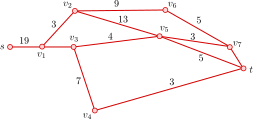
\includegraphics[width=\textwidth]{graph}

\paragraph{Answer}

\todo{replace this TODO with your answer}
%%%%%%%%%%%%%%%%%%%%%%%%%%%%%%%%%%%%%%%%%%%%%%%%%%%%%%%%%%%%%%%%%%%%%%%%%%%%%%

%%%%%%%%%%%%%%%%%%%%%%%%%%%%%%%%%%%%%%%%%%%%%%%%%%%%%%%%%%%%%%%%%%%%%%%%%%%%%%
\collab{\todo{}}
\nextprob{ARTISOIL}

Chapter 3, Problem 2a.

\paragraph{Answer}

\todo{replace this TODO with your answer}
%%%%%%%%%%%%%%%%%%%%%%%%%%%%%%%%%%%%%%%%%%%%%%%%%%%%%%%%%%%%%%%%%%%%%%%%%%%%%%

\end{document}
